\section{Methodology}

\subsection{Research Design and Methodological Framework}

This study was designed as a controlled ablation study for supervised rice leaf disease classification. The methodological framework follows an applied quantitative experimental approach: a computational pipeline was implemented, the input-processing configuration was deliberately modified across experimental scenarios, and the resulting models were compared using numerical performance and efficiency metrics.

The ablation design was selected to isolate the contribution of each component under comparable conditions. Instead of evaluating only a final proposed architecture, the study compared a baseline CNN, a segmentation-based variant, a texture-fusion variant, and a segmentation-texture hybrid variant. To ensure a fair comparison, all scenarios used the same dataset split, image size, training configuration, evaluation metrics, and random seeds. Therefore, the intended experimental factor was the presence or absence of segmentation and explicit texture descriptors.

\subsection{Dataset and Split Distribution}

The experiments used the Rice Leaf Disease Images dataset, organized into four disease classes: Bacterial Blight, Blast, Brown Spot, and Tungro. The final dataset contained 5,932 images. The dataset was divided into training, validation, and test sets following an approximate 70\%--15\%--15\% distribution. The training set contained 4,150 images, representing 69.96\% of the dataset; the validation set contained 891 images, representing 15.02\%; and the test set contained 891 images, also representing 15.02\%. Table~\ref{tab:split_distribution} shows the final class distribution.

\begin{table}[t]
\caption{Dataset split distribution by class.}
\label{tab:split_distribution}
\centering
\footnotesize
\setlength{\tabcolsep}{4pt}
\begin{tabular}{lccc}
\toprule
Class & Train & Val. & Test \\
\midrule
Bacterial Blight & 1108 & 238 & 238 \\
Blast            & 1007 & 216 & 217 \\
Brown Spot       & 1120 & 241 & 239 \\
Tungro           & 915  & 196 & 197 \\
\midrule
Total            & 4150 & 891 & 891 \\
Percentage       & 69.96\% & 15.02\% & 15.02\% \\
\bottomrule
\end{tabular}
\end{table}

\subsection{Data Leakage Control Using Perceptual Hashing}

A preliminary inspection showed that the dataset contained visually repeated or highly similar samples. To reduce the risk of data leakage, the final partition was generated using perceptual hash grouping. Each image was assigned a perceptual hash, and images sharing the same hash were kept within the same split.

After this correction, the dataset contained 2,927 unique perceptual hashes across 5,932 images. The number of perceptual hashes appearing in more than one split was zero. This procedure was applied before training to avoid inflated validation or test performance caused by visually equivalent samples shared across training, validation, and test subsets.

\subsection{Experimental Scenarios}

Four scenarios were evaluated. E0 was the baseline model trained with original RGB images. E1 evaluated the effect of replacing the original RGB image with its segmented version. E2 evaluated the effect of fusing MobileNetV2 image embeddings with explicit GLCM+DWT features extracted from original images. E3 was the proposed hybrid variant, combining segmented images with GLCM+DWT features extracted from the segmented image source. Table~\ref{tab:scenarios} summarizes the four ablation scenarios evaluated in the study.

\begin{table}[t]
\caption{Ablation scenarios evaluated in the study.}
\label{tab:scenarios}
\centering
\footnotesize
\setlength{\tabcolsep}{3pt}
\begin{tabularx}{\columnwidth}{c X X}
\toprule
ID & Configuration & Purpose \\
\midrule
E0 & MobileNetV2 + original RGB image & Baseline \\
E1 & MobileNetV2 + segmented image & Segmentation effect \\
E2 & MobileNetV2 + original image + GLCM+DWT & Texture fusion effect \\
E3 & MobileNetV2 + segmented image + GLCM+DWT & Proposed hybrid variant \\
\bottomrule
\end{tabularx}
\end{table}

\subsection{Evaluation Protocol}

The primary evaluation metric was macro-F1, selected because it gives equal importance to all classes. Additional metrics included accuracy, macro-precision, macro-recall, confusion matrix, inference time per image, number of parameters, and model size.

To evaluate stability, the complete training process was repeated using five random seeds: 42, 123, 2026, 7, and 99. This produced 20 total runs, corresponding to four experimental scenarios evaluated across five seeds. Final performance was summarized using the mean and standard deviation across seeds.

Since the same seeds were used for all scenarios, pairwise differences against the baseline were computed by seed. The Wilcoxon signed-rank test was used to assess whether the macro-F1 differences between each enhanced scenario and the baseline were statistically significant without assuming normality of the paired differences.

Figure~\ref{fig:experimental_framework} summarizes the complete experimental workflow, including dataset preparation, leakage control, ablation scenarios, model training, evaluation metrics, and comparative analysis.

\begin{figure*}[!t]
\centering
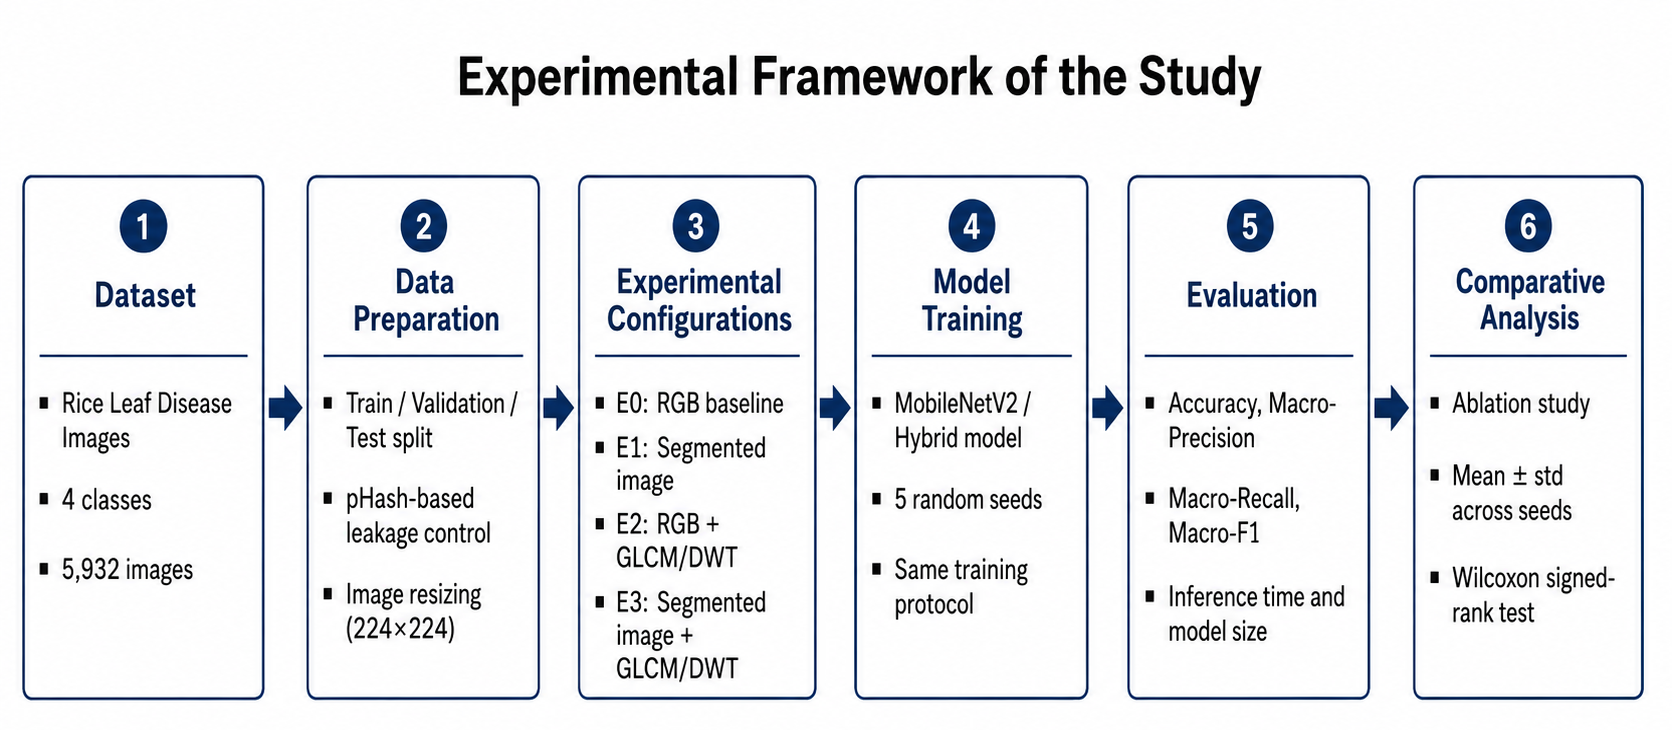
\includegraphics[width=0.88\textwidth]{figures/fig01_experimental_framework.png}
\caption{Experimental framework and ablation scenarios evaluated in this study.}
\label{fig:experimental_framework}
\end{figure*}
